\chapter{Application and validation}

After the theoretical basis of the virtual experiment platform is known and 
the program of the virtual experiment platform is built, the application should be 
verified with experiment data generated based on the real experiment.


\begin{figure}[htbp]
    \centering
    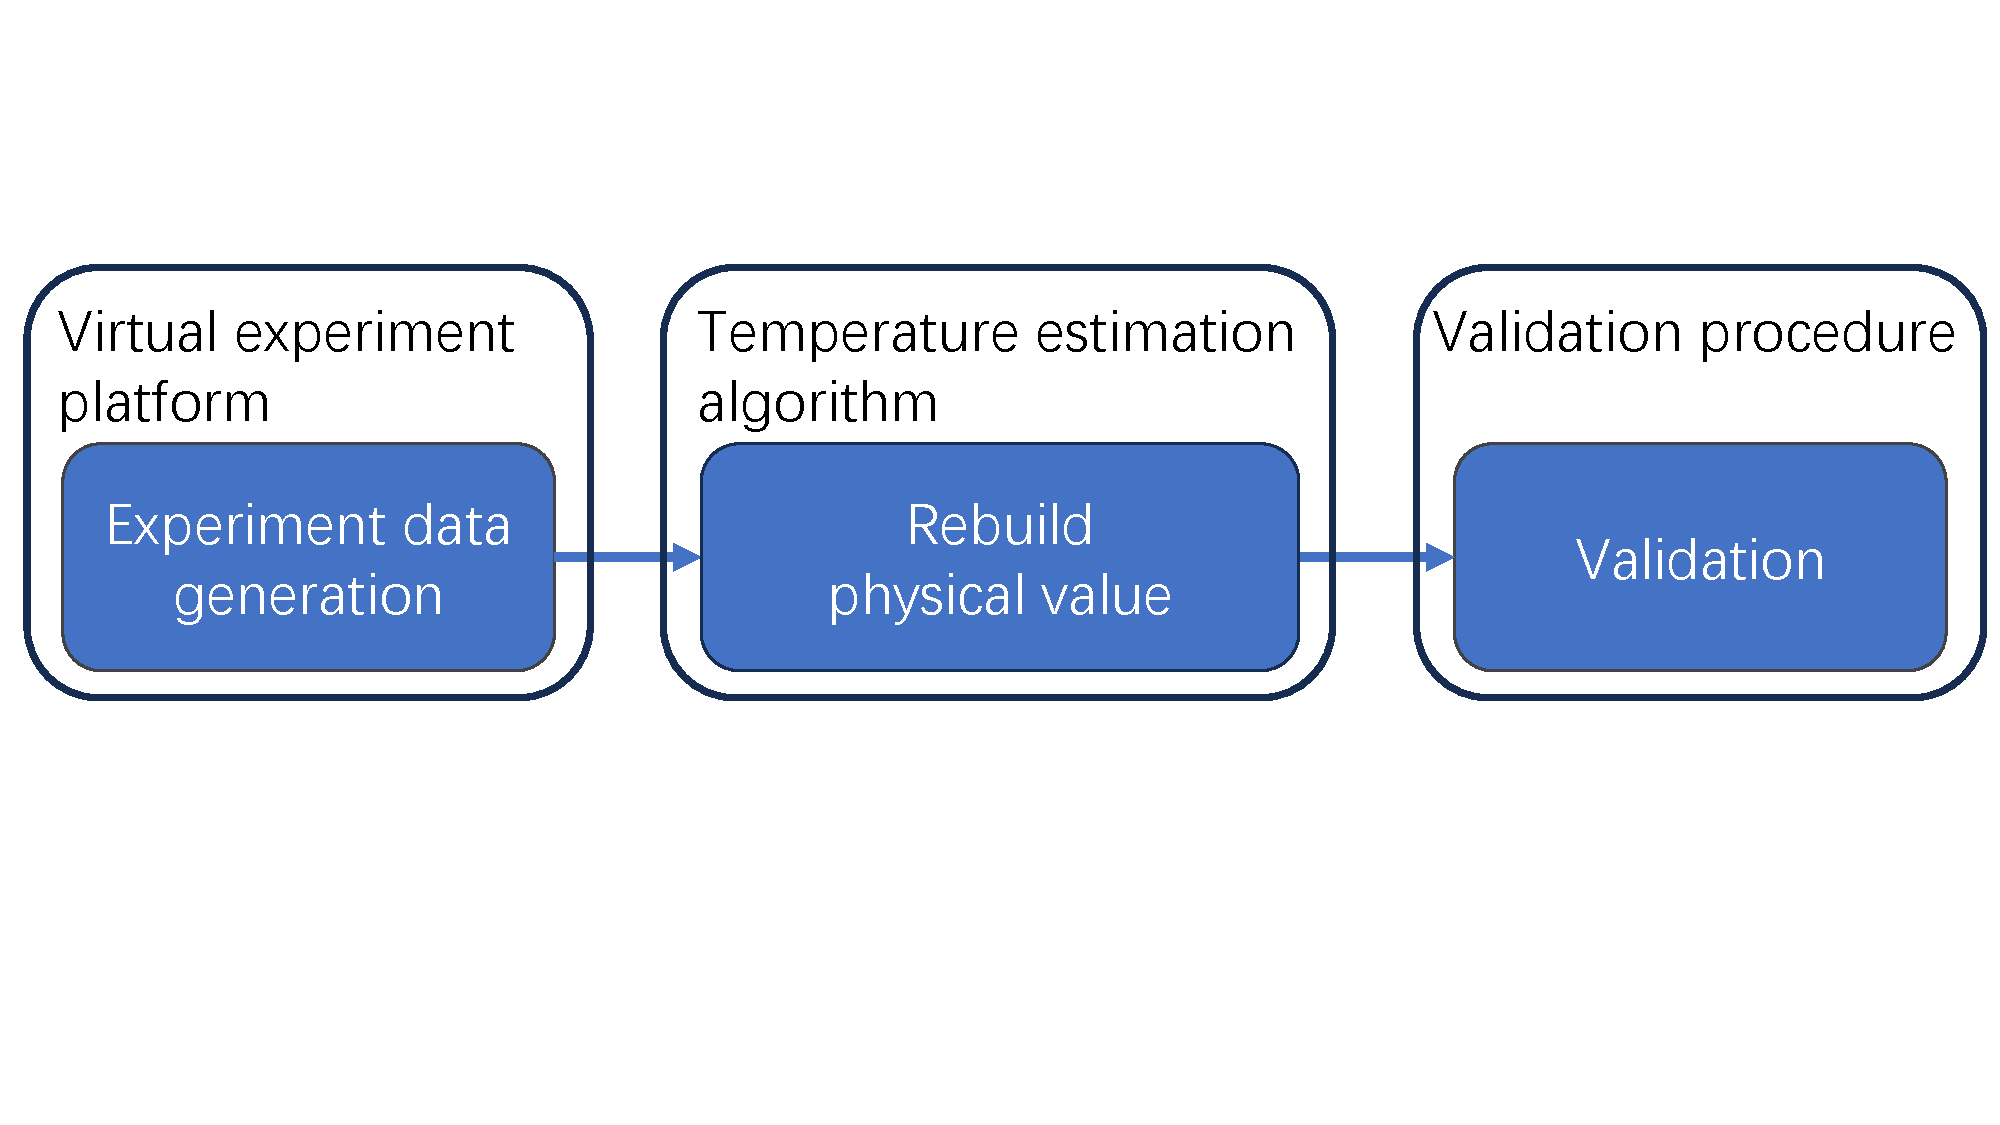
\includegraphics[width=0.90\textwidth]{figures/application_procedure.pdf}
    \caption{Complete procedure from data generation to model validation}
    \label{fig: application_procedure}
\end{figure}


Fig.\ref{fig: application_procedure} shows the procedure of the application.
Firstly, an experiment data set should be generated according to the parameters of the 
hypothetical material. Then, a temperature estimation algorithm is applied to 
estimate the temperature of the hypothetical material. Last, a validation procedure 
is used to check the accuracy and stability of the results of 
temperature estimation algorithm.


As mentioned in previous sections, these functions is implemented in three 
programmes. Namely virtual experiment platform, temperature estimation algorithm
and validation procedure. Similar to conventional experiment methods, these
steps are independent procedures, which means they do not interact with 
each other. 


Accordingly, this chapter will be divided into three sections, which describe 
the implementation and the parameter settings of the virtual experiment platform, 
temperature estimation algorithm and validation procedure.


\section{Experiment data generation}
As the first of the three steps mentioned above, it is crucial to generate 
accurate experimental data correctly. It affects the comparability of the 
virtual experimental platform with real experiments on the one hand, and 
the accuracy of the temperature estimation algorithm on the other. As a 
result, the virtual experimental platform should be able to perform 
calculations for as many hypothetical materials with different properties 
as possible.


In order to be able to obtain image similar to image from
real camera, the area that the virtual camera is able to capture is 
set to a 50*50 pixel picture. Fig.\ref{fig: camera} shows the image obtained 
from real experiment and virtual experiment platform. The major difference between 
these two images is the coloring. In real experiment, the raw image was saved 
as a .tiff file, which obtain the spectral intensity received by the specific 
channel. Then, the intensity is expressed as brightness of the pixel in the display of 
the image. This results in the experiment data that is not intuitive and 
requires specialised software to open these data.


As a result, there are a number of optimisations that have been applied 
in this virtual experiment platform. Firstly, the raw digital value 
of the received spectral intensity was saved in an .xlsx file, which 
simplifies the reading of the data as well as the conversion. In 
addition, a .jpg image of each channel similar to the real experiment data is also 
saved. Different from the real experiment data, colours are used here to 
indicate the value of the spectral intensity. This improves the 
readability of the experiment data.


\begin{figure}[htbp]
    \centering
    \begin{subfigure}{0.45\textwidth}
        \centering
        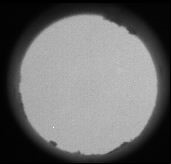
\includegraphics[height=5cm]{figures/real_camera_1075.JPG}
        \caption{Real experiment data  (channel 1)}
        \label{fig: real_camera}
    \end{subfigure}
    % \hfill
    \begin{subfigure}{0.45\textwidth}
        \centering
        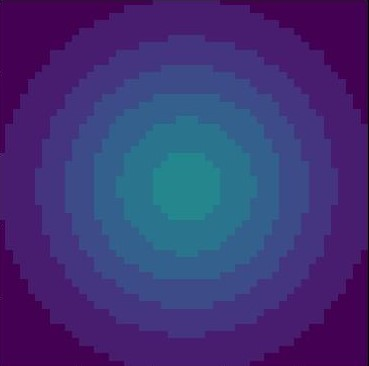
\includegraphics[height=5cm]{figures/virtual_camera_1098.jpg}
        \caption{Virtual experiment data (channel 1)}
        \label{fig: virtual_camera}
    \end{subfigure}
    \caption{Comparison between real experiment data at $1300K$ (a)
    and virtual experiment data at $1098K$ (b)
    }
    \label{fig: camera}
\end{figure}


Thus, the observation area is obtained by initialization of the the virtual 
experiment platform. Temperature field, emissivity model of the hypothetical 
material and the integration method are the parameters to be defined as the next
step.


\subsection{Temperature field}%
\subsection{Emissivity model}%
\subsection{Integration method}
\section{Rebuild Physical value}
\subsection{Emissivity model used for calculation}

\subsection{Curve fit algorithm}

\subsection{Parameters in calculation}
quantum efficiency, lens factor

\section{Validation}